% !TeX spellcheck = en_US
\documentclass[a4paper]{scrartcl}

\usepackage[utf8]{inputenc}
\usepackage[english]{babel}
\usepackage[T1]{fontenc}
\usepackage{lmodern}
\usepackage{amsmath}
\usepackage{amssymb}
\usepackage{pdflscape}
\usepackage{geometry}
\usepackage{xcolor}
\usepackage{graphicx}
\usepackage{todonotes}
\setlength{\parindent}{0pt}

\usepackage{biblatex}
\addbibresource{references.bib}


%\geometry{a4paper, top=25mm, left=30mm, right=20mm, bottom=30mm,
%headsep=10mm, footskip=12mm}

\newcommand{\itab}[1]{\hspace{0em}\rlap{#1}}
\newcommand{\tab}[1]{\hspace{.2\textwidth}\rlap{#1}}
\newcommand{\asd}[1]{\textbf{#1}}

\title{All different types of digram types from Maneth and Peternek}
\author{Matthias Dürksen}
\date{\today}
 

\begin{document}
\maketitle
\section*{Purpose of the document}
This document provides an overview of the different types of digrams described in the Maneth paper.
The nodes have been labeled in contrast to Maneth and equivalence classes for nodes have been added. The Digram types of Maneth and Peternek are therefore not necessarily directly applicable to the approach of our graph compression.

\section{Maneth's digrams}


Incident edges to internal nodes are also a problem here. This is solved by Maneth's approach by using a new digram rule where the incident edges are contained in the digram. So instead of simple edges hyper edges are created. This is illustrated in Figure ~\ref{fig:type1}.




    

\begin{figure}[h]
	\centering
	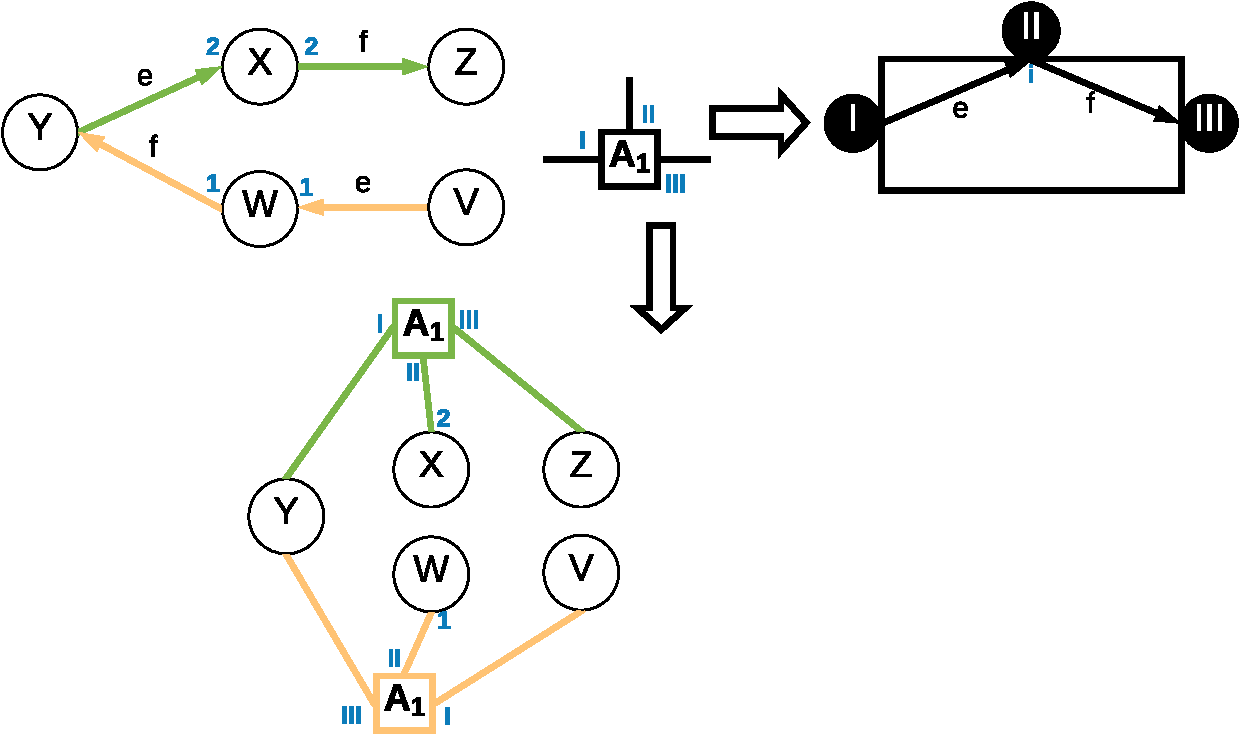
\includegraphics[width=0.7\textwidth]{img/type1}
	\caption{Application of a replacement of one digram type}
	\label{fig:type1}
\end{figure}

\begin{figure}[h]
	\centering
	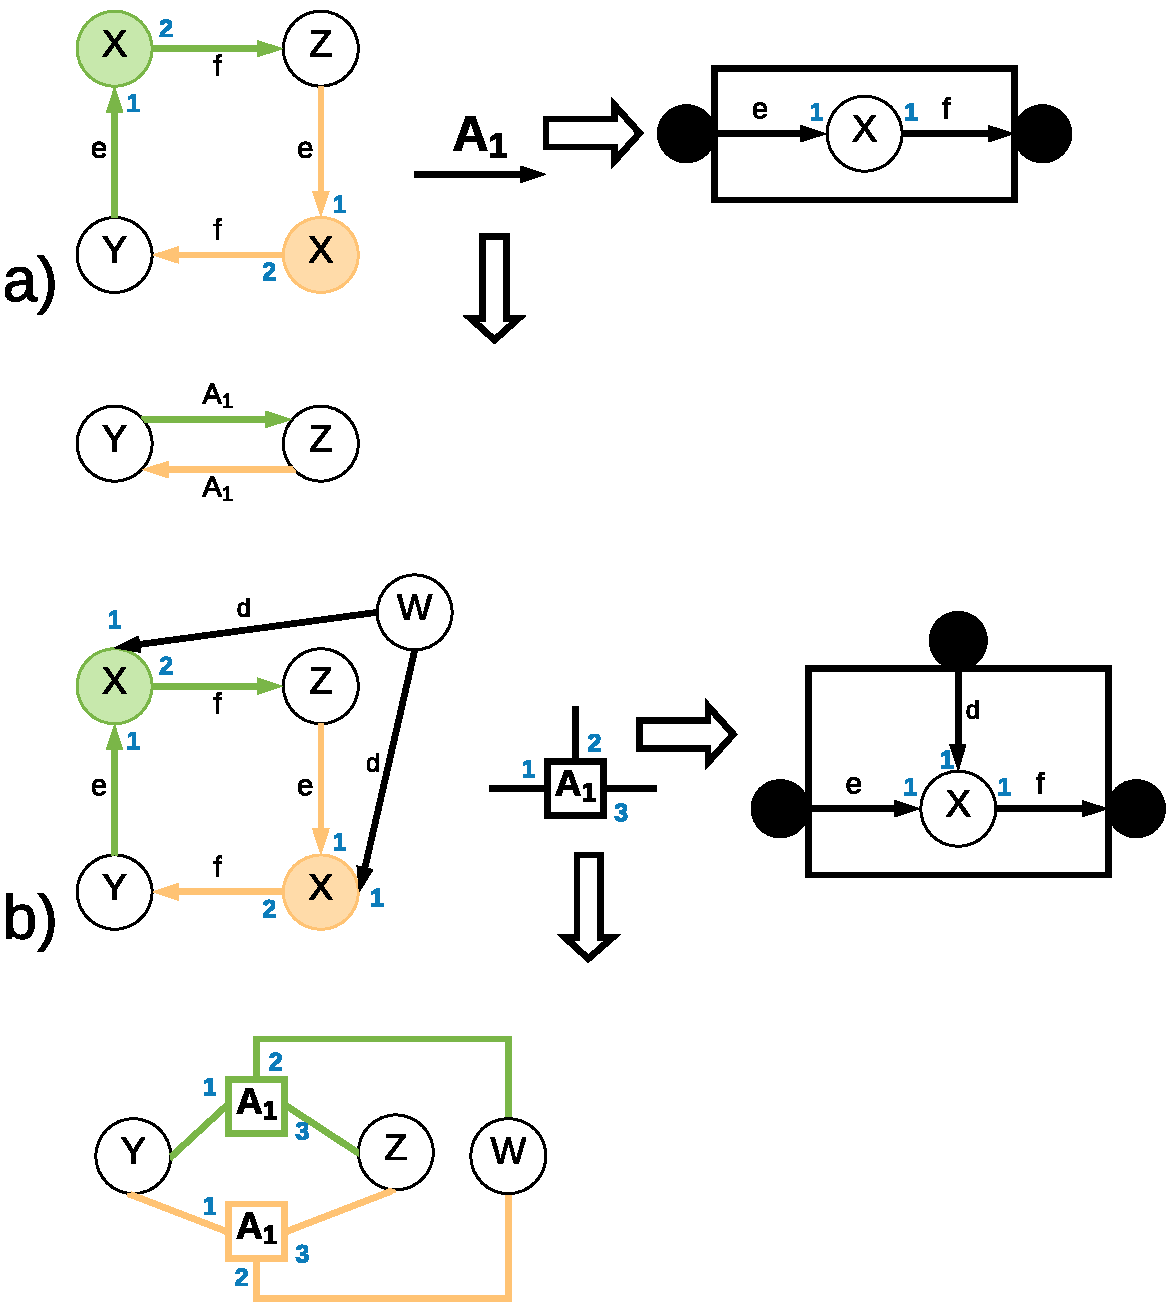
\includegraphics[width=0.7\textwidth]{img/type2}
	\caption{Application of a replacement of one digram type}
	\label{fig:type2}
\end{figure}

\begin{figure}[h]
	\centering
	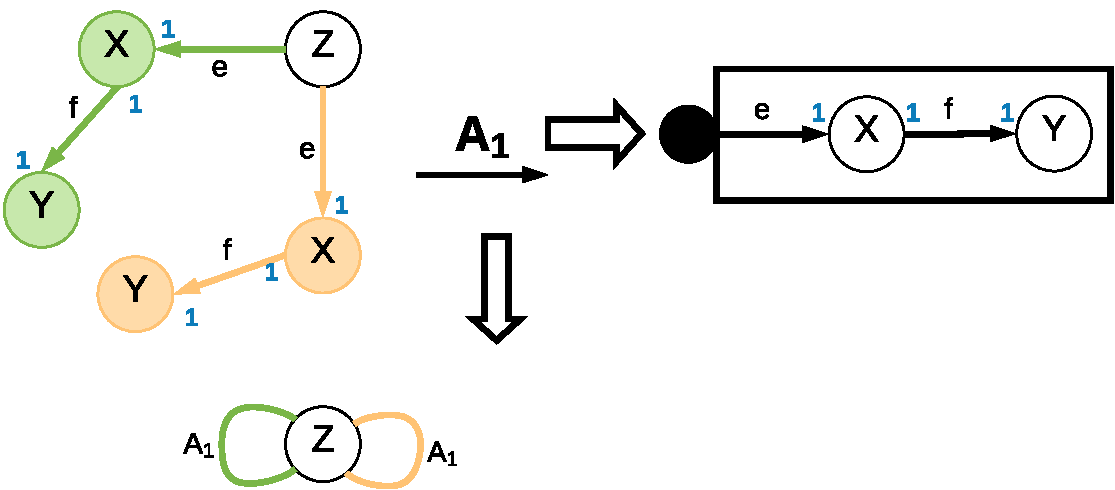
\includegraphics[width=0.7\textwidth]{img/type3}
	\caption{Application of a replacement of one digram type}
	\label{fig:type3}
\end{figure}

\begin{figure}[h]
	\centering
	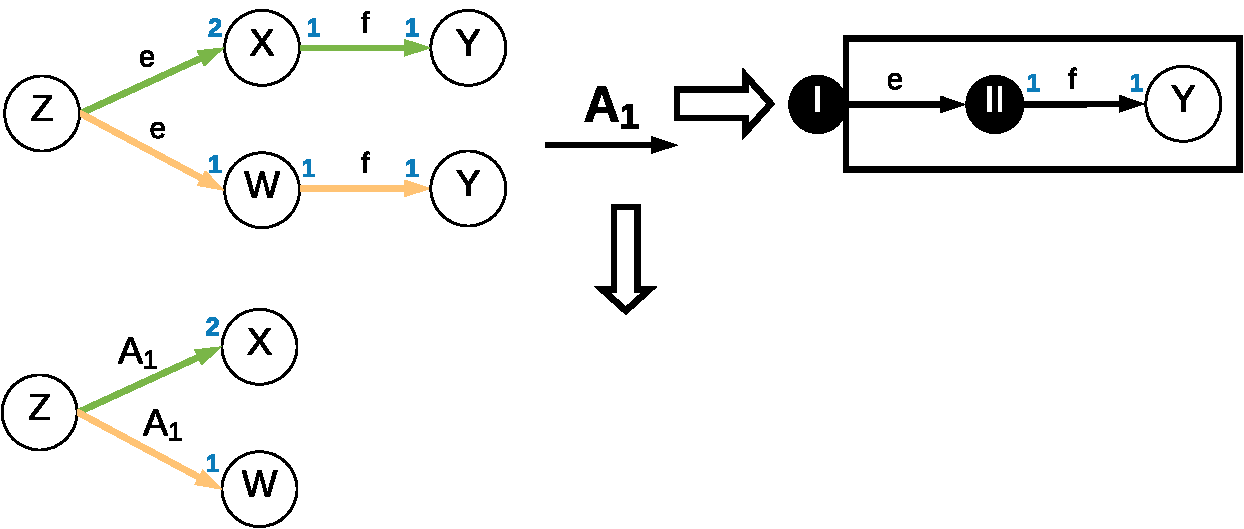
\includegraphics[width=0.7\textwidth]{img/type4}
	\caption{Application of a replacement of one digram type}
	\label{fig:type4}
\end{figure}

\begin{figure}[h]
	\centering
	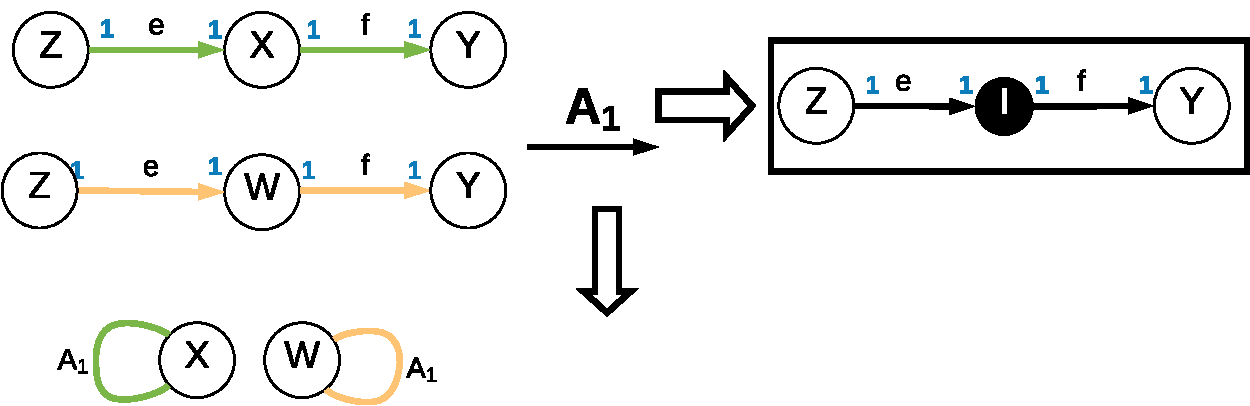
\includegraphics[width=0.7\textwidth]{img/type5}
	\caption{Application of a replacement of one digram type}
	\label{fig:type5}
\end{figure}

\begin{figure}[h]
	\centering
	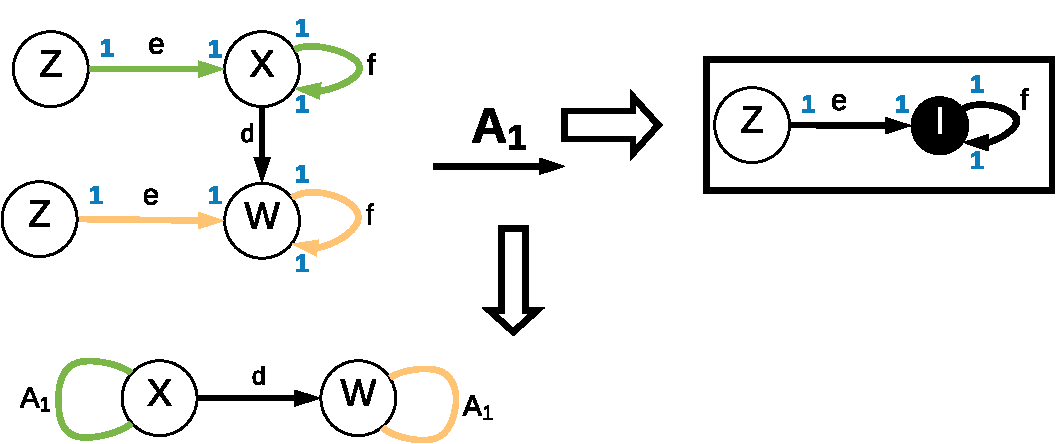
\includegraphics[width=0.7\textwidth]{img/type6}
	\caption{Application of a replacement of one digram type}
	\label{fig:type6}
\end{figure}


\begin{figure}[h]
	\centering
	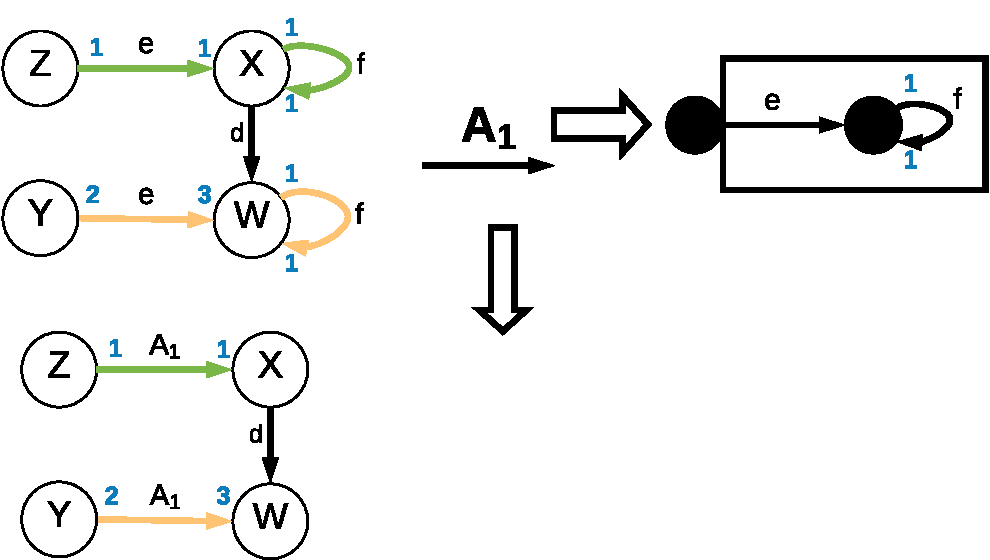
\includegraphics[width=0.7\textwidth]{img/type7}
	\caption{Application of a replacement of one digram type}
	\label{fig:type7}
\end{figure}

\begin{figure}[h]
	\centering
	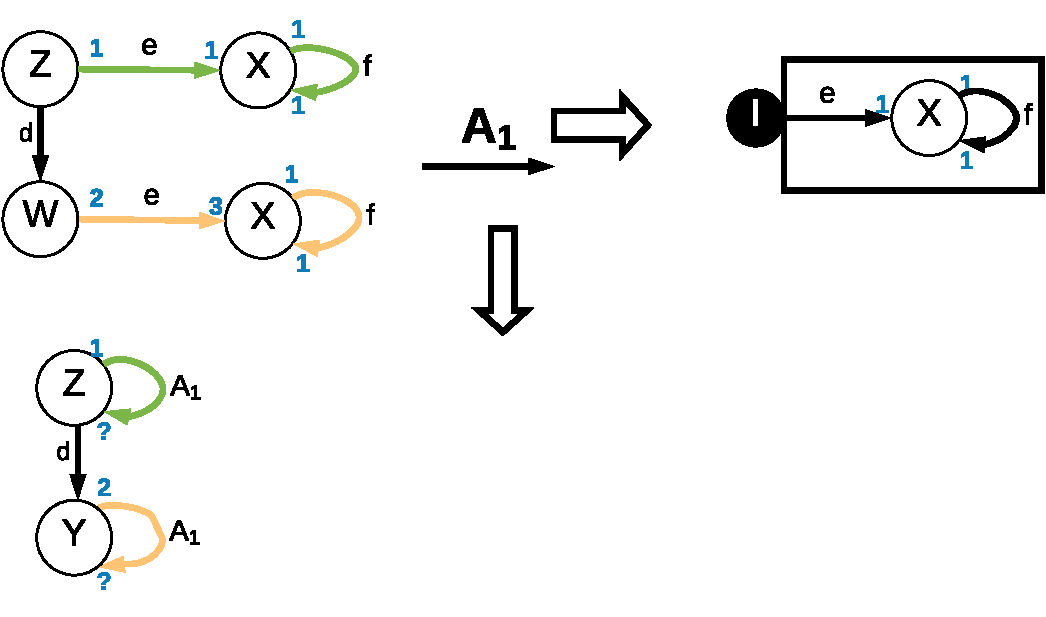
\includegraphics[width=0.7\textwidth]{img/type8}
	\caption{Application of a replacement of one digram type}
	\label{fig:type8}
\end{figure}

\begin{figure}[h]
	\centering
	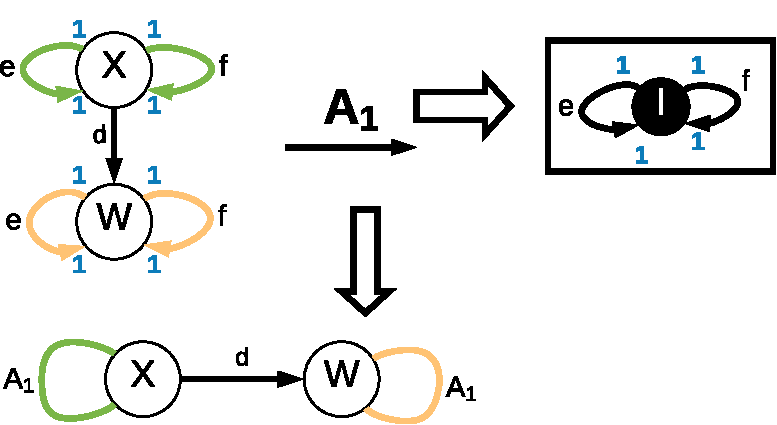
\includegraphics[width=0.7\textwidth]{img/type9}
	\caption{Application of a replacement of one digram type}
	\label{fig:type9}
\end{figure}











\pagebreak
%\printbibliography







\end{document}